\documentclass[border=5pt]{standalone}
\usepackage{pgfplots}
\usepackage{tikz}
\usepackage{textcomp}
\usepackage{comment}

\begin{document}

% Plotting mathematical expressions

    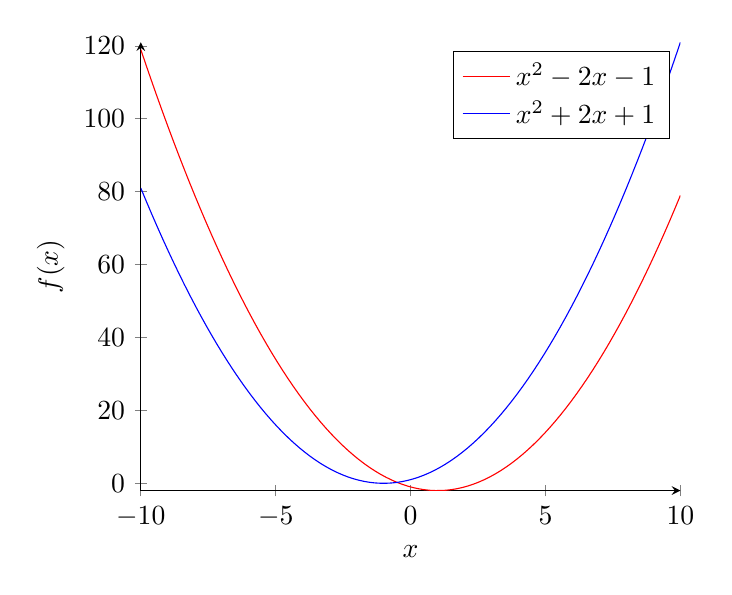
\begin{tikzpicture}
        \begin{axis}[
            axis lines = left,
            xlabel = $x$,
            ylabel = {$f(x)$},
        ]
        %Below the red parabola is defined
        \addplot [
            domain=-10:10, 
            samples=100, 
            color=red,
        ]
        {x^2 - 2*x - 1};
        \addlegendentry{$x^2 - 2x - 1$}
        %Here the blue parabloa is defined
        \addplot [
            domain=-10:10, 
            samples=100, 
            color=blue,
            ]
            {x^2 + 2*x + 1};
        \addlegendentry{$x^2 + 2x + 1$}
         
        \end{axis}
    \end{tikzpicture}

% Plotting from data

    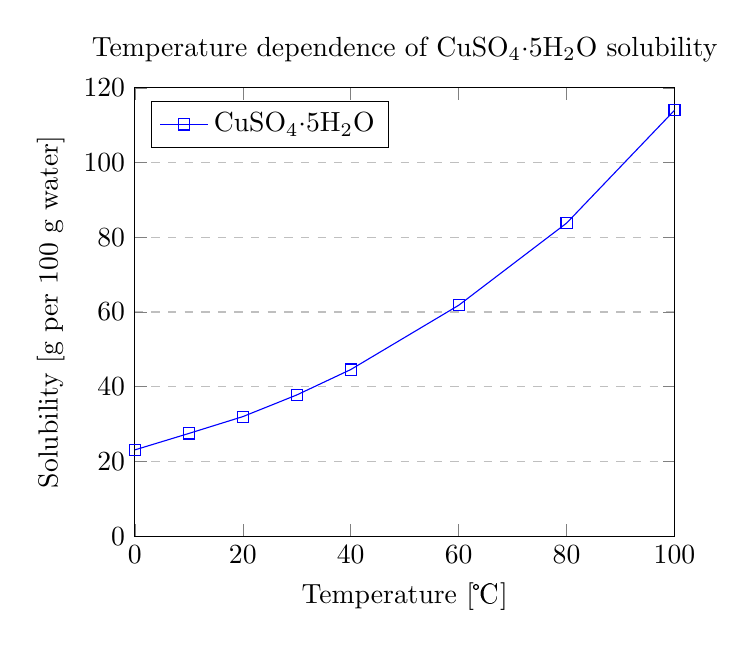
\begin{tikzpicture}
        \begin{axis}[
            title={Temperature dependence of CuSO$_4\cdot$5H$_2$O solubility},
            xlabel={Temperature [\textcelsius]},
            ylabel={Solubility [g per 100 g water]},
            xmin=0, xmax=100,
            ymin=0, ymax=120,
            xtick={0,20,40,60,80,100},
            ytick={0,20,40,60,80,100,120},
            legend pos=north west,
            ymajorgrids=true,
            grid style=dashed,
        ]
         
        \addplot[
            color=blue,
            mark=square,
            ]
            coordinates {
            (0,23.1)(10,27.5)(20,32)(30,37.8)(40,44.6)(60,61.8)(80,83.8)(100,114)
            };
            \legend{CuSO$_4\cdot$5H$_2$O}
         
        \end{axis}
    \end{tikzpicture}

% Scatter Plot

    \begin{tikzpicture}
        \begin{axis}[
            enlargelimits=false,
        ]
        \addplot+[
            only marks,
            scatter,
            mark=halfcircle*,
            mark size=2.9pt]
        table[meta=ma]
        {scattered_example.dat};
        \end{axis}
    \end{tikzpicture}

% Bar graphs

    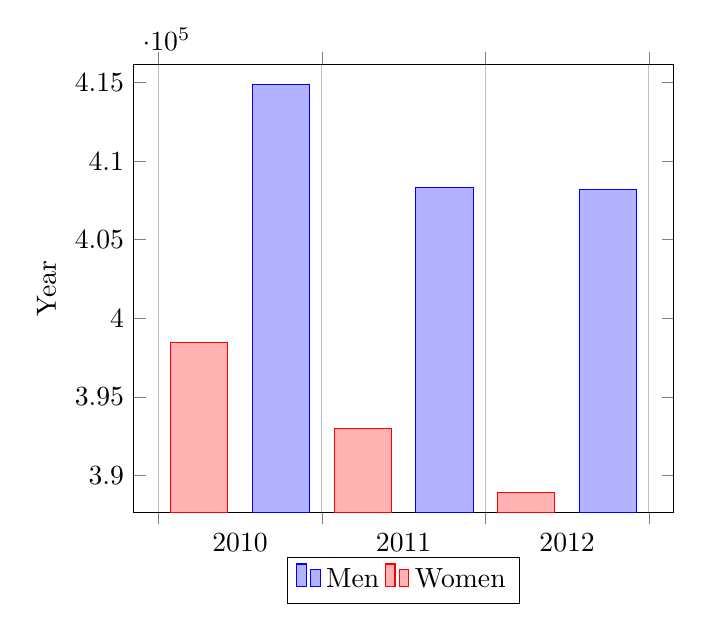
\begin{tikzpicture}
        \begin{axis}[
            x tick label style={
                /pgf/number format/1000 sep=},
            ylabel=Year,
            enlargelimits=0.05,
            legend style={at={(0.5,-0.1)},
            anchor=north,legend columns=-1},
            ybar interval=0.7,
        ]
        \addplot 
            coordinates {(2012,408184) (2011,408348)
                 (2010,414870) (2009,412156)};
        \addplot 
            coordinates {(2012,388950) (2011,393007) 
                (2010,398449) (2009,395972)};
        \legend{Men,Women}
        \end{axis}
    \end{tikzpicture}

% 3D Plot

    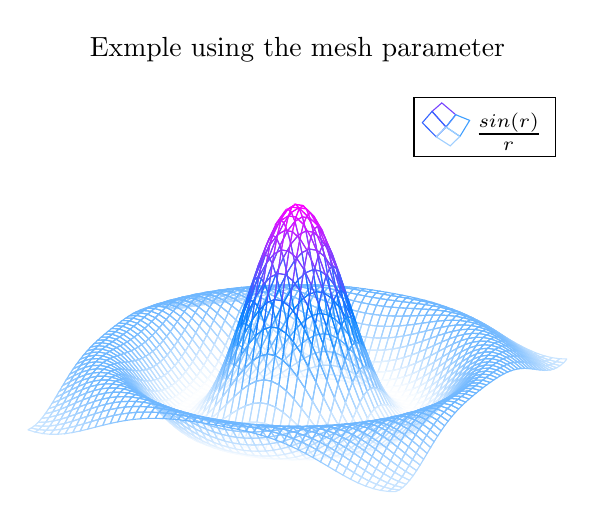
\begin{tikzpicture}
        \begin{axis}[
            title=Exmple using the mesh parameter,
            hide axis,
            colormap/cool,
        ]
        \addplot3[
            mesh,
            samples=50,
            domain=-8:8,
        ]
        {sin(deg(sqrt(x^2+y^2)))/sqrt(x^2+y^2)};
        \addlegendentry{$\frac{sin(r)}{r}$}
        \end{axis}
    \end{tikzpicture}

% Contour plots

\begin{comment}
     \begin{tikzpicture}
        \begin{axis}
        [
            title={Contour plot, view from top},
            view={0}{90}
        ]
        \addplot3[
            contour gnuplot={levels={0.8, 0.4, 0.2, -0.2}}
        ]
        {sin(deg(sqrt(x^2+y^2)))/sqrt(x^2+y^2)};
        \end{axis}
    \end{tikzpicture}
\end{comment}
\end{document}
